\documentclass[a4paper,12pt]{article}
\usepackage[utf8x]{inputenc}
\usepackage[english]{babel}
\usepackage[T1]{fontenc}
\usepackage{times}
\usepackage{graphicx}
\usepackage{float}
\usepackage{subfig}
\usepackage[top=2cm, bottom=2cm, left=2.5cm, right=2.5cm]{geometry}

\title{You's Social Network}
\date{\today}

\begin{document}

\maketitle


\begin{figure}[H]
\centering
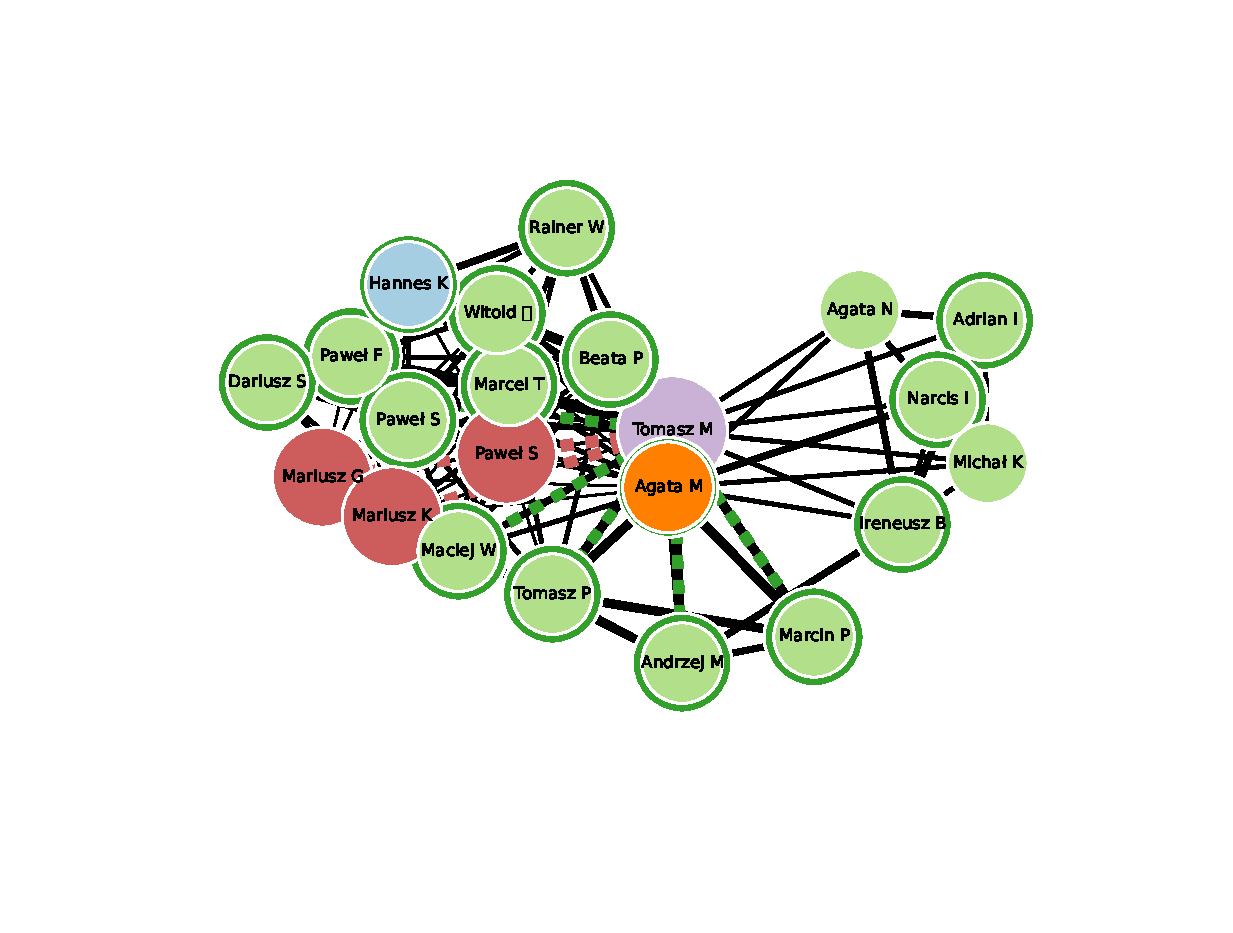
\includegraphics[scale=0.5]{/home/jtorrents/projects/egosite/media/egoreports/1_7adca287-4241-496f-96b4-1d5bcdf2a6ea/acebcb33-e80c-497b-81ec-a1874b089e74/egonet_kk}
\end{figure}


\tableofcontents
\newpage


Thinking about your social network might help you go beyond a simplistic view of what your contacts are (who do you know?) and help you think about how the people in your company are connected to each other (your indirect contacts). The patterns of relations among people in your company, and your concrete position in those patterns, might allow you to access and procure valuable intangible assets, such as good advice, technical knowledge, emotional support, etc.

This report is based on the confidential information on your contact network collected with the web-based survey that you just completed. We analyzed your network to evaluate how your network may help you access important assets and organize them to achieve your professional goals. To improve the interpretation of your results, we compare them with the results of the other people in your group.

The report is organized in three parts. First, we analyze your network in terms of the number and the diversity of your contacts. Second, we analyze your network in terms of the kind and the strength of the relationships between you and your contacts. Third, we analyze the structure of your network, focusing on the patterns of relations among your contacts.


\section{Your Contacts}


The diversity of the attributes of the people that forms your personal social network is a source of different perspectives that can allow you to find innovative solutions to the problems that you face at work. However, it might also increase coordination costs and thus hinder action and decision making.


\begin{figure}[H]
\centering
\subfloat[Your personal results]{\includegraphics[scale=0.3]{/home/jtorrents/projects/egosite/media/egoreports/1_7adca287-4241-496f-96b4-1d5bcdf2a6ea/acebcb33-e80c-497b-81ec-a1874b089e74/gender}}
\hspace{.01in}
\subfloat[Average of your group results]{\includegraphics[scale=0.3]{/home/jtorrents/projects/egosite/media/egoreports/1_7adca287-4241-496f-96b4-1d5bcdf2a6ea/average/gender}}
\caption{This chart shows the gender distribution of your contacts. Gender diversity reveals your exposure to the view-points and experiences of the different sexes. This is partly defined by demographics since there are still significantly more men than women in most business settings. But it can be also driven by stereotypes: some men may find it difficult to build good professional relationships with women (and vice-versa).}
\end{figure}


\begin{figure}[H]
\centering
\subfloat[Your personal results]{\includegraphics[scale=0.3]{/home/jtorrents/projects/egosite/media/egoreports/1_7adca287-4241-496f-96b4-1d5bcdf2a6ea/acebcb33-e80c-497b-81ec-a1874b089e74/age}}
\hspace{.01in}
\subfloat[Average of your group results]{\includegraphics[scale=0.3]{/home/jtorrents/projects/egosite/media/egoreports/1_7adca287-4241-496f-96b4-1d5bcdf2a6ea/average/age}}
\caption{This graph illustrates the distribution of your contacts by age. The age of your contacts is important because different generations have gone through different experiences that configure their opinions and their attitudes. The age of our contacts typically increases with age. This is natural, but also has draw-backs. A network can be a bridge across generations or it may amplify the natural separation between them.}
\end{figure}


\begin{figure}[H]
\centering
\subfloat[Your personal results]{\includegraphics[scale=0.3]{/home/jtorrents/projects/egosite/media/egoreports/1_7adca287-4241-496f-96b4-1d5bcdf2a6ea/acebcb33-e80c-497b-81ec-a1874b089e74/work}}
\hspace{.01in}
\subfloat[Average of your group results]{\includegraphics[scale=0.3]{/home/jtorrents/projects/egosite/media/egoreports/1_7adca287-4241-496f-96b4-1d5bcdf2a6ea/average/work}}
\caption{The graph above shows the proportion of contacts working in your same unit, in your same function (but in a different unit), in your same firm (but in a different function), and in other firms. It indicates the extent to which your network is limited to your own firm or office.}
\end{figure}


\begin{figure}[H]
\centering
\subfloat[Your personal results]{\includegraphics[scale=0.3]{/home/jtorrents/projects/egosite/media/egoreports/1_7adca287-4241-496f-96b4-1d5bcdf2a6ea/acebcb33-e80c-497b-81ec-a1874b089e74/rank}}
\hspace{.01in}
\subfloat[Average of your group results]{\includegraphics[scale=0.3]{/home/jtorrents/projects/egosite/media/egoreports/1_7adca287-4241-496f-96b4-1d5bcdf2a6ea/average/rank}}
\caption{The chart looks at the hierarchical diversity of your network. The diversity is your network in terms of rank is partly dependent on your own rank.}
\end{figure}


\begin{figure}[H]
\centering
\subfloat[Your personal results]{\includegraphics[scale=0.3]{/home/jtorrents/projects/egosite/media/egoreports/1_7adca287-4241-496f-96b4-1d5bcdf2a6ea/acebcb33-e80c-497b-81ec-a1874b089e74/functional_area}}
\hspace{.01in}
\subfloat[Average of your group results]{\includegraphics[scale=0.3]{/home/jtorrents/projects/egosite/media/egoreports/1_7adca287-4241-496f-96b4-1d5bcdf2a6ea/average/functional_area}}
\caption{This graph illustrates the distribution of your contacts by their primary functional or professional area. It measures the extent to which your network reaches across functional boundaries. A network with contacts from different functional backgrounds exposes you to a richer picture of the business and allows you to learn about more opportunities to achieve your professional goals.}
\end{figure}


\section{Your Relations}


The quality of the relationships between you and your contacts is a good proxy of their willingness to help, and their diversity affects the extent of the resources and information they can provide. The disposition to help and the breadth of that help may be also shaped by the structure of your network.


\begin{figure}[H]
\centering
\subfloat[Your personal results]{\includegraphics[scale=0.3]{/home/jtorrents/projects/egosite/media/egoreports/1_7adca287-4241-496f-96b4-1d5bcdf2a6ea/acebcb33-e80c-497b-81ec-a1874b089e74/strength}}
\hspace{.01in}
\subfloat[Average of your group results]{\includegraphics[scale=0.3]{/home/jtorrents/projects/egosite/media/egoreports/1_7adca287-4241-496f-96b4-1d5bcdf2a6ea/average/strength}}
\caption{This graph represents the strength of the relationship with each contact in term of the closeness between you and the contact. Closer relationships might help you receive more support from your contacts.}
\end{figure}


\begin{figure}[H]
\centering
\subfloat[Your personal results]{\includegraphics[scale=0.3]{/home/jtorrents/projects/egosite/media/egoreports/1_7adca287-4241-496f-96b4-1d5bcdf2a6ea/acebcb33-e80c-497b-81ec-a1874b089e74/frequency}}
\hspace{.01in}
\subfloat[Average of your group results]{\includegraphics[scale=0.3]{/home/jtorrents/projects/egosite/media/egoreports/1_7adca287-4241-496f-96b4-1d5bcdf2a6ea/average/frequency}}
\caption{The chart displays the frequency with which you communicate with your contacts capturing your tendency to concentrate this communication on a specific time frame (e.g., on a weekly basis).}
\end{figure}


\begin{figure}[H]
\centering
\subfloat[Your personal results]{\includegraphics[scale=0.3]{/home/jtorrents/projects/egosite/media/egoreports/1_7adca287-4241-496f-96b4-1d5bcdf2a6ea/acebcb33-e80c-497b-81ec-a1874b089e74/helps}}
\hspace{.01in}
\subfloat[Average of your group results]{\includegraphics[scale=0.3]{/home/jtorrents/projects/egosite/media/egoreports/1_7adca287-4241-496f-96b4-1d5bcdf2a6ea/average/helps}}
\caption{This graph represents how helpful your contacts are and the degree of supportiveness. Contacts with whom you have a long-lasting, frequent, and emotionally close relationship know you and your needs well. They are around to help when you need it, and they are more inclined to do so than weakly tied contacts.}
\end{figure}


\begin{figure}[H]
\centering
\subfloat[Your personal results]{\includegraphics[scale=0.3]{/home/jtorrents/projects/egosite/media/egoreports/1_7adca287-4241-496f-96b4-1d5bcdf2a6ea/acebcb33-e80c-497b-81ec-a1874b089e74/context}}
\hspace{.01in}
\subfloat[Average of your group results]{\includegraphics[scale=0.3]{/home/jtorrents/projects/egosite/media/egoreports/1_7adca287-4241-496f-96b4-1d5bcdf2a6ea/average/context}}
\caption{This chart looks at the origin of your relationships. If most of our contacts come from one single source it is more likely that they will be similar in other aspects too.}
\end{figure}


\section{Structure of your social network}


\subsection{Mapping your social network}


One picture is worth a thousand words, and you might get a better sense for where you are in the company if you try to position yourself in its social graph. Looking at the connections among people that you are directly connected with can provide useful insight. For instance, you might realize you happen to work as the link between otherwise disconnected others, thus being able to bridge the gap among different groups, receiving knowledge and information from all of them and controlling to some extent the information flow among them.


\begin{figure}[H]
\centering
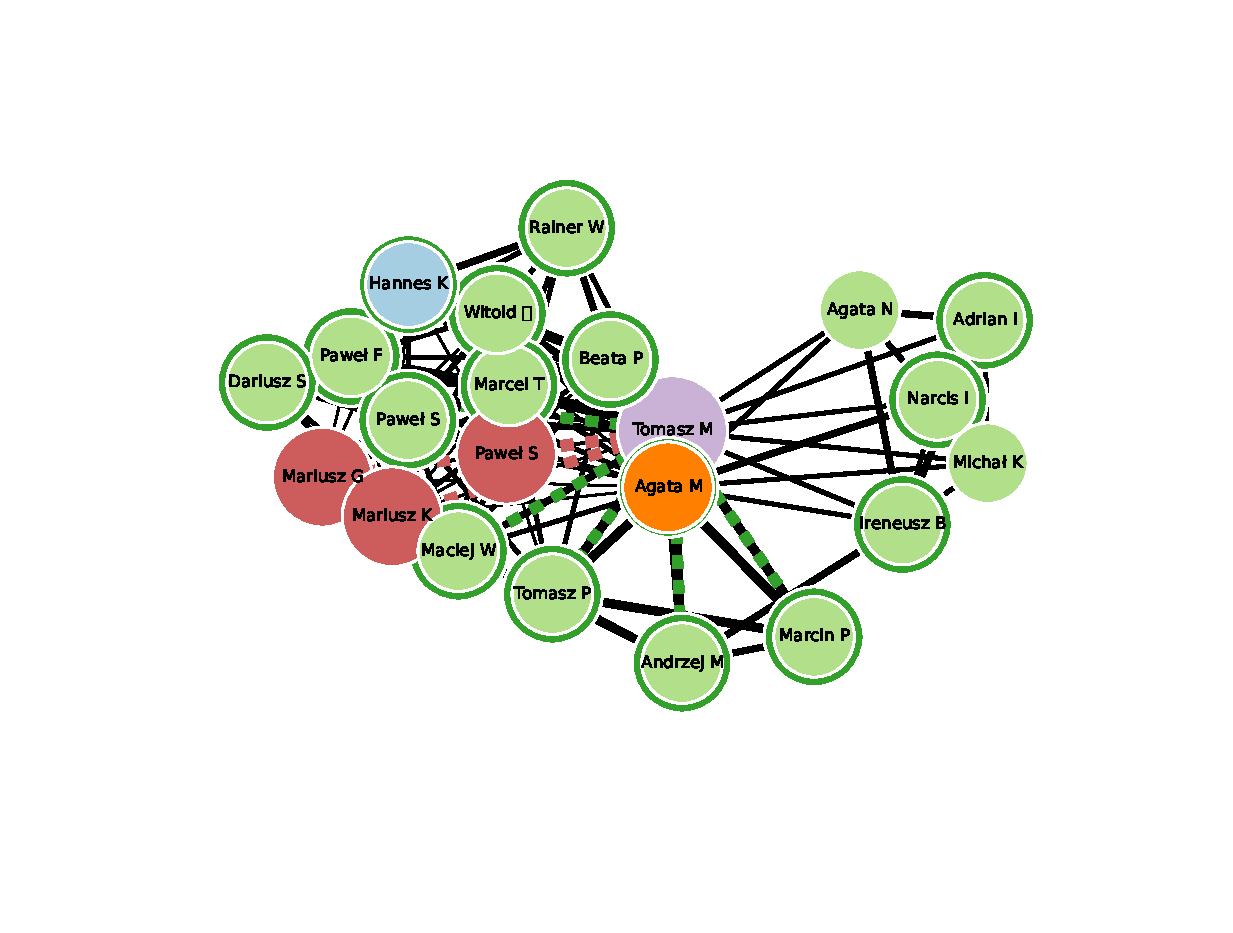
\includegraphics[scale=0.7]{/home/jtorrents/projects/egosite/media/egoreports/1_7adca287-4241-496f-96b4-1d5bcdf2a6ea/acebcb33-e80c-497b-81ec-a1874b089e74/egonet_kk}
\caption{In this plot, you and your contacts are depicted as nodes linked through relations of different strength and nature. You are the bigger violet node. The light blue node is your boss. In red you have all the contacts with whom you maintained an adversarial relation (if any). The contacts with the green borders are the ones that help you the most. All other contacts are plotted as smaller light green nodes. The tie width represents the strength of the connection. All adversarial relations are plotted using a dashed red link.}
\end{figure}


\subsection{Density of your social network}


\begin{figure}[H]
\centering
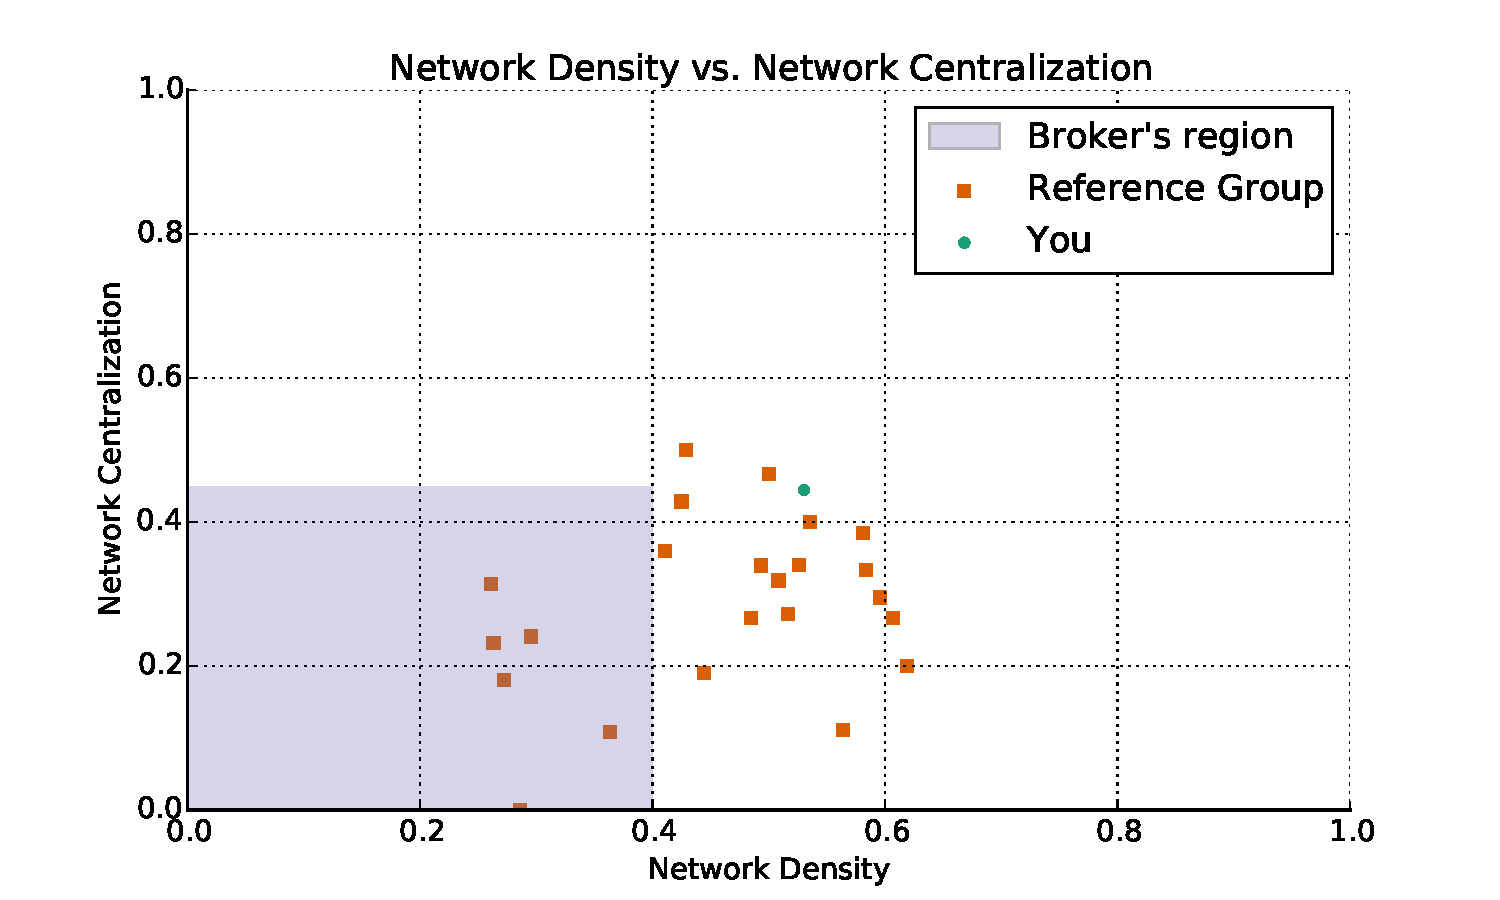
\includegraphics[scale=0.6]{/home/jtorrents/projects/egosite/media/egoreports/1_7adca287-4241-496f-96b4-1d5bcdf2a6ea/acebcb33-e80c-497b-81ec-a1874b089e74/density_cent}
\caption{Network centralization vs. network density. The chart above plots both your results and the ones of the other survey respondents using their density and centralization scores. Density measures the proportion of direct ties in a network relative to the total number possible. The higher the centralization of your network, the more your network connectivity depends on one or few nodes that are connected with most people around you. The denser the network, the more all your contacts are connected with one another, and therefore your network is less likely to be centralized.}
\end{figure}


\end{document}

